\chapter{RISC-V 迁移与测试验证}

\section{迁移总体思路}

本课题的架构迁移不是对原有代码逐行改写，而是在保留原系统教学逻辑的前提下重建底层体系结构相关部分。迁移路径包括 Sv39 分页适配、串口和块设备驱动迁移、文件系统 I/O 路径接入以及系统测试。

这一路径的约束来自原系统本身。IA32 版本的页表、PIC 中断控制器和 ATA 设备接口都直接嵌入启动、内存管理和块 I/O 路径；迁移到 RISC-V 后，对应部分变为 Sv39 三级页表、RISC-V trap 入口、PLIC 外部中断控制器以及 VirtIO MMIO 块设备。若只替换汇编指令和寄存器访问，上层文件系统仍无法获得稳定的块读写接口，用户进程也不能在新的页表布局下运行。因此，本章关注的不是指令层面的翻译，而是平台相关边界的重建。

具体实现按照依赖关系推进。启动初期先保留尽可能少的运行条件，只保证 Rust 入口、串口输出和分页前后的控制流切换可见；随后建立 Sv39 页表，使内核高地址映射、用户低地址映射和 MMIO 区域各自落在确定的地址范围内；在此基础上接入 UART 和 VirtIO 块设备，再恢复文件系统装载、控制台打开、init 进程创建和 shell 运行。这样的顺序也便于定位故障，启动错误通常暴露在串口输出之前，页表错误多出现在地址切换后，块设备错误则会在超级块读取和用户程序加载阶段出现。

迁移过程中特别需要控制修改边界。内存管理和文件系统已经在 Rust 版本中重新组织，如果 RISC-V 分支同时大幅改写 inode、目录解析或打开文件表，就很难判断故障来自架构适配还是来自上层算法变化。因此，RISC-V 版本把主要改动限定在启动、页表、trap、MMIO 和块设备接口处，尽量复用前面已经稳定下来的文件系统主路径。这样处理虽然不能一次性覆盖所有平台特性，但有利于把“跨架构能否复用”作为一个可验证的问题。

\section{RISC-V 内存管理适配实现}

RISC-V 版本的虚拟内存以 Sv39 为基础。Sv39 使用三级页表，每级页表包含 512 个表项，页大小为 4KB，虚拟地址被拆分为三级索引和页内偏移。与 IA32 版本相比，Sv39 的页表层次和权限位较少依赖历史兼容设计，页表项中的 VALID、READ、WRITE、EXECUTE、USER 等标志可以直接对应映射是否有效、能否读写执行以及是否允许用户态访问。

代码中没有把页表项作为裸整数在各处拆解，而是以结构体承载页框号和标志位，并通过 EntryFlags 封装 VALID、READ、WRITE、EXECUTE、USER、ACCESSED 和 DIRTY 等权限。分页开启时，内核把根页表物理页号写入 satp，并将模式设置为 Sv39；写入后立即刷新 TLB，避免切换前残留的地址转换结果影响后续访问。

地址空间仍沿用“内核位于高地址、用户空间位于低地址”的教学组织方式，但具体边界按 RISC-V virt 平台重新设置。物理内存从 RAM\_BASE 开始，内核虚拟地址从 KERNEL\_VIRT\_BASE 开始；UART、PLIC 和 VirtIO 不再混在普通 RAM 映射中，而是放入高地址 MMIO 区域。这样处理后，访问普通内存、内核符号和设备寄存器时使用的地址范围可以从代码层面区分出来。

用户空间仍然位于低地址区域，并由固定数量的用户页表覆盖。代码中使用 4 个用户页表，构成统一的用户地址空间上界。MemoryDescriptor 负责管理用户进程的代码段、数据段和栈段映射，并在需要时把逻辑布局映射到实际页表中。

页表初始化没有采用运行时按需分配的复杂策略，而是预先维护根页目录、低地址目录、内核恒等映射目录、内核高地址目录和内核页表等静态对象。启动阶段先清空这些页表，再写入内核恒等映射、高地址内核映射和用户页表数组。内核空间具备两套映射后，代码才能安全地完成从物理地址执行到高地址执行的切换。

对于用户空间，系统在初始化阶段预留用户页表数组，并在进程运行过程中由 MemoryDescriptor 将具体的代码段、数据段和栈段映射到对应页表项。进程切换时，系统更新当前进程用户结构所在页的映射，并刷新 TLB，以保证内核能够访问当前进程的用户态上下文。

Sv39 适配中最容易出错的是地址阶段切换。启动早期代码通常运行在物理地址或恒等映射条件下，分页启用后同一段内核代码需要能够继续通过高地址访问自身和全局数据。为此，RISC-V 分支在开启分页前同时准备恒等映射和高地址映射，使切换前后的取指、栈访问和全局符号访问都能落到有效页表项上。MMIO 区域单独映射也服务于同一目标：普通内存页可以按缓存和权限语义管理，设备寄存器访问则被限制在明确的地址范围内，减少页表调试时不同访问类型混杂带来的干扰。

\section{设备与 I/O 子系统迁移实现}

串口路径主要用于启动日志、调试输出和 shell 输入。RISC-V 版本没有长期依赖 SBI 字符输出，而是直接访问 UART0\_BASE 所在的 MMIO 寄存器，完成波特率、8N1 格式、FIFO 和接收中断配置。发送路径采用轮询，接收路径检查就绪位后读取输入字符。该部分不是迁移工作的主要难点，但它提供了后续页表切换、文件系统装载和 shell 测试所需的可观察通道。

块设备是迁移中影响文件系统的关键差异。IA32 版本通过 ATA DMA 访问磁盘，RISC-V 版本改用 VirtIO MMIO。当前实现由 VirtIOBlockDriver 扫描若干 MMIO 槽位，识别设备类型为块设备的 VirtIO 设备，再交给 \texttt{virtio-drivers} 完成传输队列初始化和块请求提交。

在数据传输过程中，驱动根据缓冲区中的块号、传输长度和读写标志调用 \texttt{read\_blocks} 或 \texttt{write\_blocks}。同时，为了适配 VirtIO 驱动框架，还实现了专门的 VirtioHal 接口，用于完成 DMA 页分配、MMIO 地址映射和共享缓冲区处理。DMA 页由内核页分配器提供，物理地址和内核虚拟地址之间的转换则通过内存管理模块统一完成。

文件系统上层没有感知 ATA 到 VirtIO 的替换。inode 读写、超级块装载和用户程序加载仍然通过统一的块设备接口发起请求；差异被限制在块设备实现和 MMIO 映射层。这个结果也反向检验了前面重构出的模块边界，文件系统依赖的是“能按块读写的设备”，而不是某一种具体控制器。

VirtIO 路径还暴露出一个与 IA32 版本不同的资源关系。ATA DMA 路径主要围绕控制器寄存器和 PRD 表组织请求，VirtIO 则要求驱动、设备和共享缓冲区之间遵守描述符队列协议。共享缓冲区既要能被内核虚拟地址访问，也要向设备提供可识别的物理地址，因此它同时依赖页分配器、地址转换函数和 MMIO 映射。前面把页资源、物理地址和块设备接口拆开后，RISC-V 分支可以在 VirtioHal 中集中处理这些转换，而不用让文件系统层直接理解 VirtIO 描述符。

从代码差异看，RISC-V 分支主要新增或替换的是页表、trap、串口和 VirtIO 路径，文件系统内部的目录解析、块映射和 inode 管理没有随架构迁移重新设计。这种取舍降低了迁移范围，也使后续测试结果可以区分“文件系统上层算法”与“底层平台适配”两类因素。

\par
迁移工作完成后，仍需通过测试确认两类问题：内存管理和文件系统重构是否破坏原有教学功能，RISC-V 版本是否能在新的页表和块设备路径下复用上层文件系统逻辑。基于这一目的，本节只保留与主路径相关的功能测试和三个微基准测试，不展开与本文核心工作关系较弱的外设和命令覆盖。

\section{测试方案设计}

本章使用功能测试和微基准测试检查三个版本的运行状态。测试对象分别为 main 分支的 C++ + IA32 版本、refactor/x86 分支的 Rust + IA32 版本，以及 refactor/riscv 分支的 Rust + RISC-V 版本。三者均在 QEMU 中运行，测试结论只用于比较本课题关注的内存管理、文件系统和块 I/O 路径，不把结果外推到真实硬件。

测试环境统一控制以下条件：

\begin{enumerate}
  \item QEMU 版本；
  \item 宿主机硬件与操作系统环境；
  \item 虚拟机分配内存大小；
  \item 编译优化选项与编译器版本。
\end{enumerate}

\begin{table}[htbp]
  \centering
  \caption{测试环境说明}
  \begin{tabular}{p{0.20\textwidth}p{0.20\textwidth}p{0.20\textwidth}p{0.20\textwidth}}
    \toprule
    \textbf{测试环境} & \textbf{C++ + IA32} & \textbf{Rust + IA32} & \textbf{Rust + RISC-V} \\
    \midrule
    宿主机操作系统 & Windows 11 专业版 & Windows 11 专业版 & Windows 11 专业版 \\
    QEMU 运行环境 & WSL2 & WSL2 & WSL2 \\
    QEMU 版本 & i386 6.2.0 & i386 6.2.0 & riscv64 10.0.2 \\
    QEMU 分配内存大小 & 128MB & 128MB & 128MB \\
    编译器版本 & g++ 11.4.0 & rustc 1.96.0-nightly & rustc 1.96.0-nightly \\
    编译选项 & 无编译优化 & \texttt{--release} & \texttt{--release} \\
    \bottomrule
  \end{tabular}
\end{table}

性能测试使用仓库 \texttt{programs/} 目录下的三个用户态程序。 \texttt{syscall\_bench.c} 循环执行 open/close、read、seek、stat 和 write，用 \texttt{times()} 记录前后 tick 并换算平均耗时；\texttt{malloc\_bench.c} 对不同大小的内存块重复执行 malloc/free，用于观察用户态动态分配接口在小对象和接近页大小对象上的差异；\texttt{io\_throughput.c} 反复读取源文件并写入目标文件，按总传输字节数估算吞吐率。

需要说明的是，Unix V6++ 的计时来自 60Hz 系统 tick，单个 tick 约为 16.67ms。测试程序把多次循环摊薄为微秒值，但其精度受循环次数、缓存状态和调度时机影响较大。因此，表中数据更适合观察数量级和相对变化，不适合作为硬件级延迟。原始 C++ 版本暂不支持本次 malloc 测试所需的用户态动态分配接口，内存分配部分只比较两个 Rust 版本。

\section{功能测试}

功能测试不追求覆盖所有异常分支，而是先确认系统能否走完课程实验中最常使用的路径。测试内容包括页分配与用户空间增长、文件创建与删除、文件打开与关闭、文件读写、目录创建与路径解析、控制台输入输出，以及 shell 在连续执行命令后的状态保持。测试过程中使用 ls、cat、mkdir、forks 等已有用户程序，并结合新增测试程序检查文件系统和内存分配接口。

从截图和终端输出看，Rust + IA32 版本可以完成原教学系统中的基本文件操作和用户程序执行；Rust + RISC-V 版本可以完成串口初始化、文件系统装载、shell 运行和块设备读写。对本文而言，关键点在于两个 Rust 版本都能够从页分配、文件系统路径解析继续走到块设备读写，说明内存管理和文件系统重构没有破坏系统主路径。

\begin{figure}[htbp]
  \centering
  \begin{subfigure}[b]{0.46\textwidth}
    \centering
    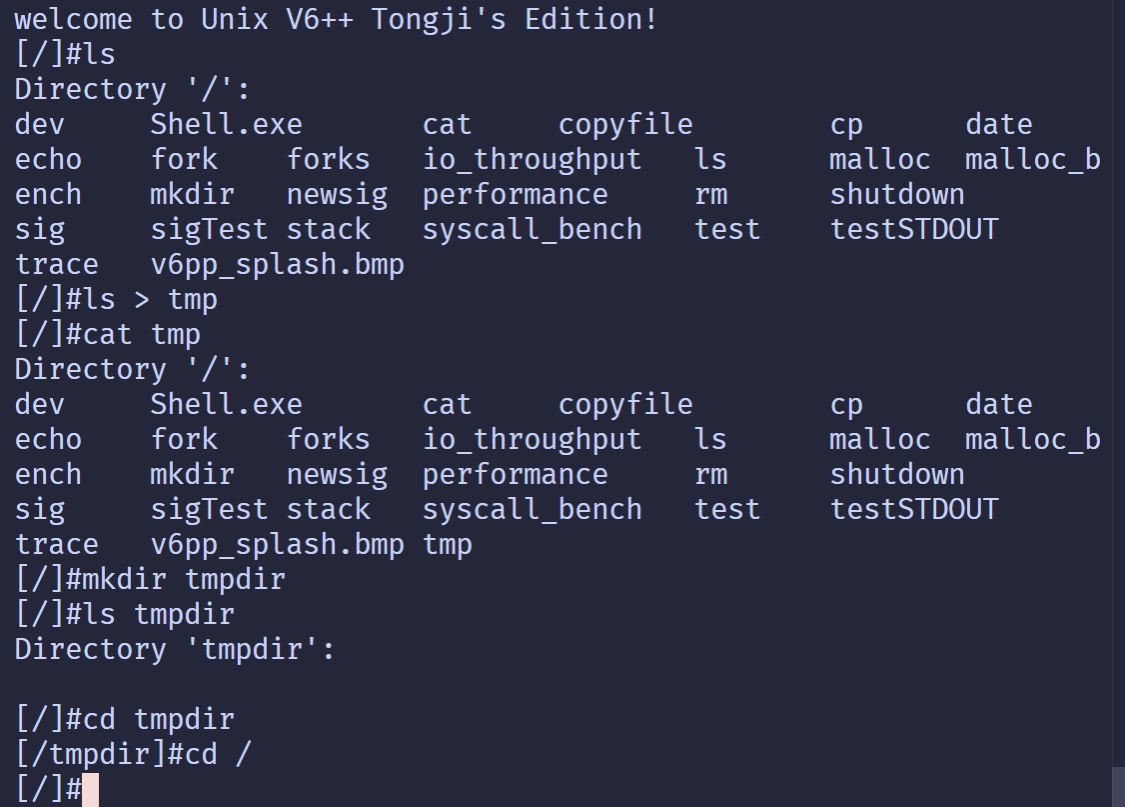
\includegraphics[width=\textwidth]{figures/7/riscv-1.png}
  \end{subfigure}
  \hfill
  \begin{subfigure}[b]{0.46\textwidth}
    \centering
    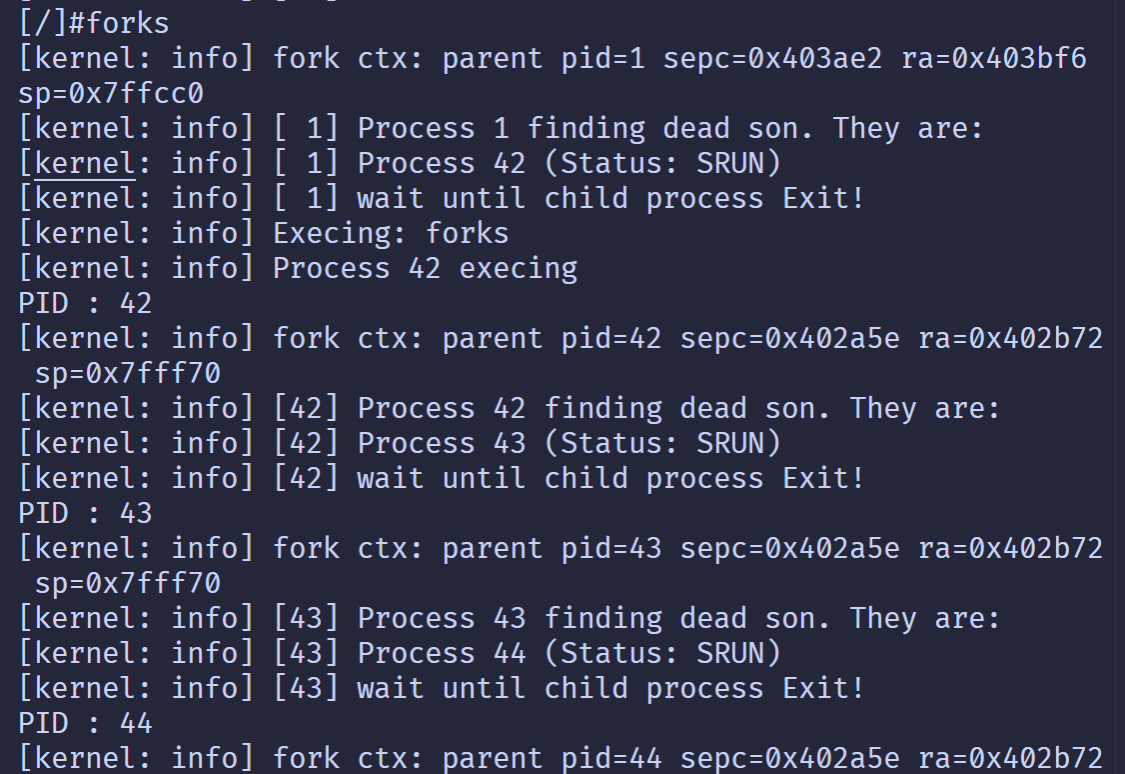
\includegraphics[width=\textwidth]{figures/7/riscv-2.png}
  \end{subfigure}
  \caption{Rust RISC-V 功能测试部分截图}
\end{figure}

\begin{figure}[htbp]
  \centering
  \begin{subfigure}[b]{0.46\textwidth}
    \centering
    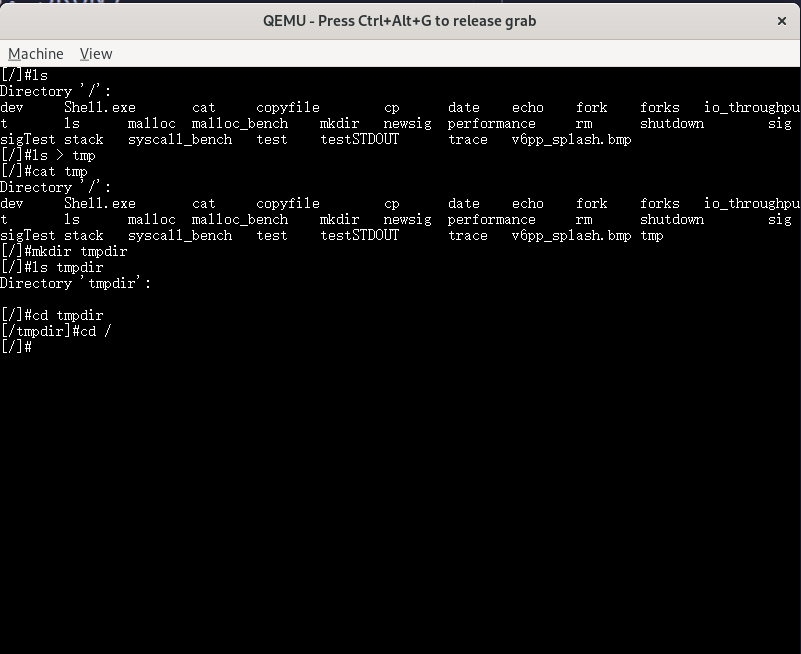
\includegraphics[width=\textwidth]{figures/7/ia32-1.png}
  \end{subfigure}
  \hfill
  \begin{subfigure}[b]{0.46\textwidth}
    \centering
    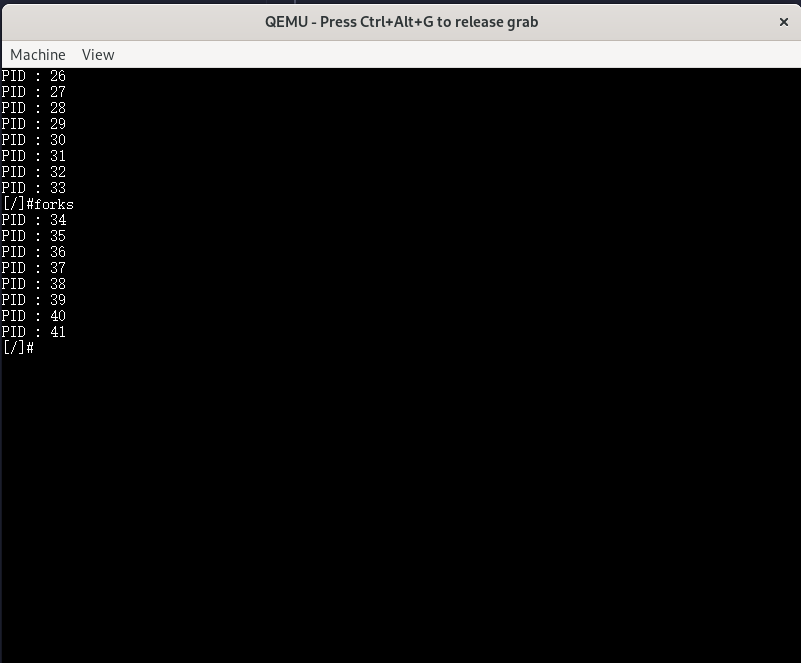
\includegraphics[width=\textwidth]{figures/7/ia32-2.png}
  \end{subfigure}
  \caption{Rust IA32 功能测试部分截图}
\end{figure}

\section{性能测试与结果分析}

系统调用延迟测试由 \texttt{syscall\_bench.c} 完成。除 write 操作固定执行 5000 次外，其余操作均执行 10000 次；读写缓冲区大小为 512 字节。测试目标文件主要为 \texttt{ls}，write 操作写入临时文件 \texttt{tmp}。由于 open/close、read、stat 与 inode 查找、打开文件表和缓冲区缓存关系较密切，这组测试可作为文件系统主路径开销的近似观察。

\begin{table}[htbp]
  \centering
  \caption{文件系统相关系统调用平均延迟（微秒/次）}\label{tab:syscall-bench}
  \begin{tabular}{p{0.20\textwidth}p{0.20\textwidth}p{0.20\textwidth}p{0.20\textwidth}}
    \toprule
    \textbf{系统调用} & \textbf{C++ + IA32} & \textbf{Rust + IA32} & \textbf{Rust + RISC-V} \\
    \midrule
    open/close & 20 & 8 & 11 \\
    read       & 25 & 6 & 6 \\
    seek       & 1  & 1 & 1 \\
    stat       & 16 & 6 & 8 \\
    write      & 103 & 90 & 106 \\
    \bottomrule
  \end{tabular}
\end{table}

内存分配测试由 \texttt{malloc\_bench.c} 完成。每种块大小下，测试程序每轮分配 20 个对象并释放，重复 50 轮，共执行 1000 次 malloc 和 1000 次 free。原始 C++ 版本暂不支持相同接口，表中以空缺标记。

\begin{table}[htbp]
  \centering
  \caption{用户态 malloc/free 平均延迟（微秒/次）}\label{tab:malloc-bench}
  \begin{tabular}{p{0.20\textwidth}p{0.20\textwidth}p{0.20\textwidth}p{0.20\textwidth}}
    \toprule
    \textbf{分配大小} & \textbf{C++ + IA32} & \textbf{Rust + IA32} & \textbf{Rust + RISC-V} \\
    \midrule
    64B   & -- & 166 & 16 \\
    128B  & -- & 166 & 16 \\
    256B  & -- & 150 & 25 \\
    512B  & -- & 158 & 50 \\
    1KB   & -- & 166 & 83 \\
    2KB   & -- & 166 & 166 \\
    4KB   & -- & 150 & 291 \\
    \bottomrule
  \end{tabular}
\end{table}

文件 I/O 吞吐量测试由 \texttt{io\_throughput.c} 完成。小文件测试以 \texttt{ls} 为源文件，重复复制 5 次；较大文件测试以 \texttt{v6pp\_splash.bmp} 为源文件，复制 1 次。小文件复制容易被缓存命中和 tick 取整放大误差，因此表中对同一版本的多次记录取平均值，只保留可比较的趋势。

\begin{table}[htbp]
  \centering
  \caption{文件 I/O 吞吐量测试结果（KB/s）}\label{tab:io-bench}
  \begin{tabular}{p{0.24\textwidth}p{0.19\textwidth}p{0.19\textwidth}p{0.19\textwidth}}
    \toprule
    \textbf{测试文件} & \textbf{C++ + IA32} & \textbf{Rust + IA32} & \textbf{Rust + RISC-V} \\
    \midrule
    \texttt{ls}，重复 5 次 & 3902 & 2503 & 2691 \\
    \texttt{v6pp\_splash.bmp}，重复 1 次 & 3409 & 4017 & 2556 \\
    \bottomrule
  \end{tabular}
\end{table}

系统调用延迟中，Rust + IA32 在 open/close、read 和 stat 上低于 C++ + IA32。这个差异不宜直接解释为“Rust 更快”，因为三组测试同时改变了代码结构、编译器、编译选项和部分实现细节。更稳妥的解释是，重构后文件对象、inode 引用和错误返回路径被集中整理，open/close 与 stat 中的表项分配、引用计数维护和失败回收更少依赖分散约定。write 的差异较小，说明写路径更多受缓冲区缓存、块设备写回和 QEMU 虚拟设备行为影响。

Rust + RISC-V 在 read、seek、stat 上与 Rust + IA32 接近，open/close 略高，write 接近 C++ + IA32。RISC-V 分支已经替换为 Sv39 页表、trap 入口和 VirtIO MMIO 块设备，而文件系统上层仍沿用同一组 inode、目录项和打开文件表逻辑。由此可以判断，迁移带来的主要差异集中在平台相关路径，文件系统核心算法没有因为架构变化而重写。

内存分配测试呈现出较清楚的大小分界。64B 至 1KB 时，Rust + RISC-V 低于 Rust + IA32；2KB 时二者接近；4KB 时 RISC-V 版本反而更高。小对象通常可以在用户态堆已取得的区域内复用，接近页大小的对象更容易触发页级分配、映射更新或空闲区管理，因此 4KB 一项的开销上升并不意外。这里不能与原始 C++ 版本直接比较，因为该版本没有跑 malloc 测试；但两个 Rust 版本的数据至少说明，RAII 封装和生命周期约束并未妨碍基本动态分配路径工作。

malloc/free 的结果还可以从页粒度解释。64B 到 1KB 的对象更多体现用户态堆内部复用能力，单次操作未必触发系统调用或新增页映射；2KB 和 4KB 的对象更接近页分配边界，测试值开始反映页表更新、空闲区维护和映射刷新等成本。由于本系统的计时粒度较粗，单个数据点不宜过度解释，但这种随对象大小变化而出现的分界与第 3 章中的 Buddy + Slab 分层设计是对应的。

文件 I/O 吞吐量需要谨慎解读。小文件测试中，C++ + IA32 平均值较高，两个 Rust 版本接近；较大位图文件测试中，Rust + IA32 较高，Rust + RISC-V 低于两个 IA32 版本。吞吐量同时受文件系统代码、QEMU 设备模型、缓存命中、块设备驱动、写回策略和 60Hz tick 取整影响。RISC-V 分支使用 VirtIO MMIO 块设备，目前更偏向先打通正确性路径，尚未针对请求合并、中断驱动传输和缓存写回策略做专门优化。

综合三组数据，本文更关注两个结论。其一，Rust 重构后，内存管理和文件系统中引入的类型化接口、RAII 风格封装和显式错误传播没有在测试范围内造成较大的开销；IA32 重构版本在若干文件系统系统调用上还低于原始版本。其二，RISC-V 版本已经能在新的页表、trap 和块设备模型下运行主要功能，但较大文件 I/O 仍受底层设备路径和模拟环境影响，后续优化应优先放在 VirtIO 请求处理和缓存策略上。

\section{本章小结}

本章比较了 C++ + IA32、Rust + IA32 和 Rust + RISC-V 三个版本。功能测试确认两个 Rust 版本均能完成文件系统装载、shell 运行、文件读写和用户程序执行。性能测试覆盖系统调用、malloc/free 和文件复制三类用户态操作。测试结果支持两个判断。内存管理和文件系统的 Rust 重构已经具备可运行性，且没有在主路径上引入明显失控的开销；RISC-V 版本已完成基本迁移，但块设备和 I/O 路径仍是后续性能优化的主要位置。
